% Provenance (never printed): cycle 2 "Questionner l'espace et le temps"
% (oceans, seas, continents on the globe) and "Questionner le monde de la
% matiere" (states of water in natural phenomena); see sources/book1/PROVENANCE.md.
% Book 1, grade 2, chapter 1.
\chapter{Air di Bumi}\label{ch:g2:water-on-earth}

Pada tanggal 7 Desember 1972, tiga astronaut yang sedang dalam perjalanan
ke Bulan mengarahkan kamera mereka kembali ke Bumi. Foto mereka menjadi
salah satu gambar paling terkenal yang pernah dibuat. Lihatlah foto itu.
Kamu bisa melihat awan putih, sedikit daratan cokelat dan kuning, es putih
di bagian bawah --- dan biru, biru di mana-mana. Dilihat dari antariksa,
planet kita adalah planet biru.

\begin{omfigure}
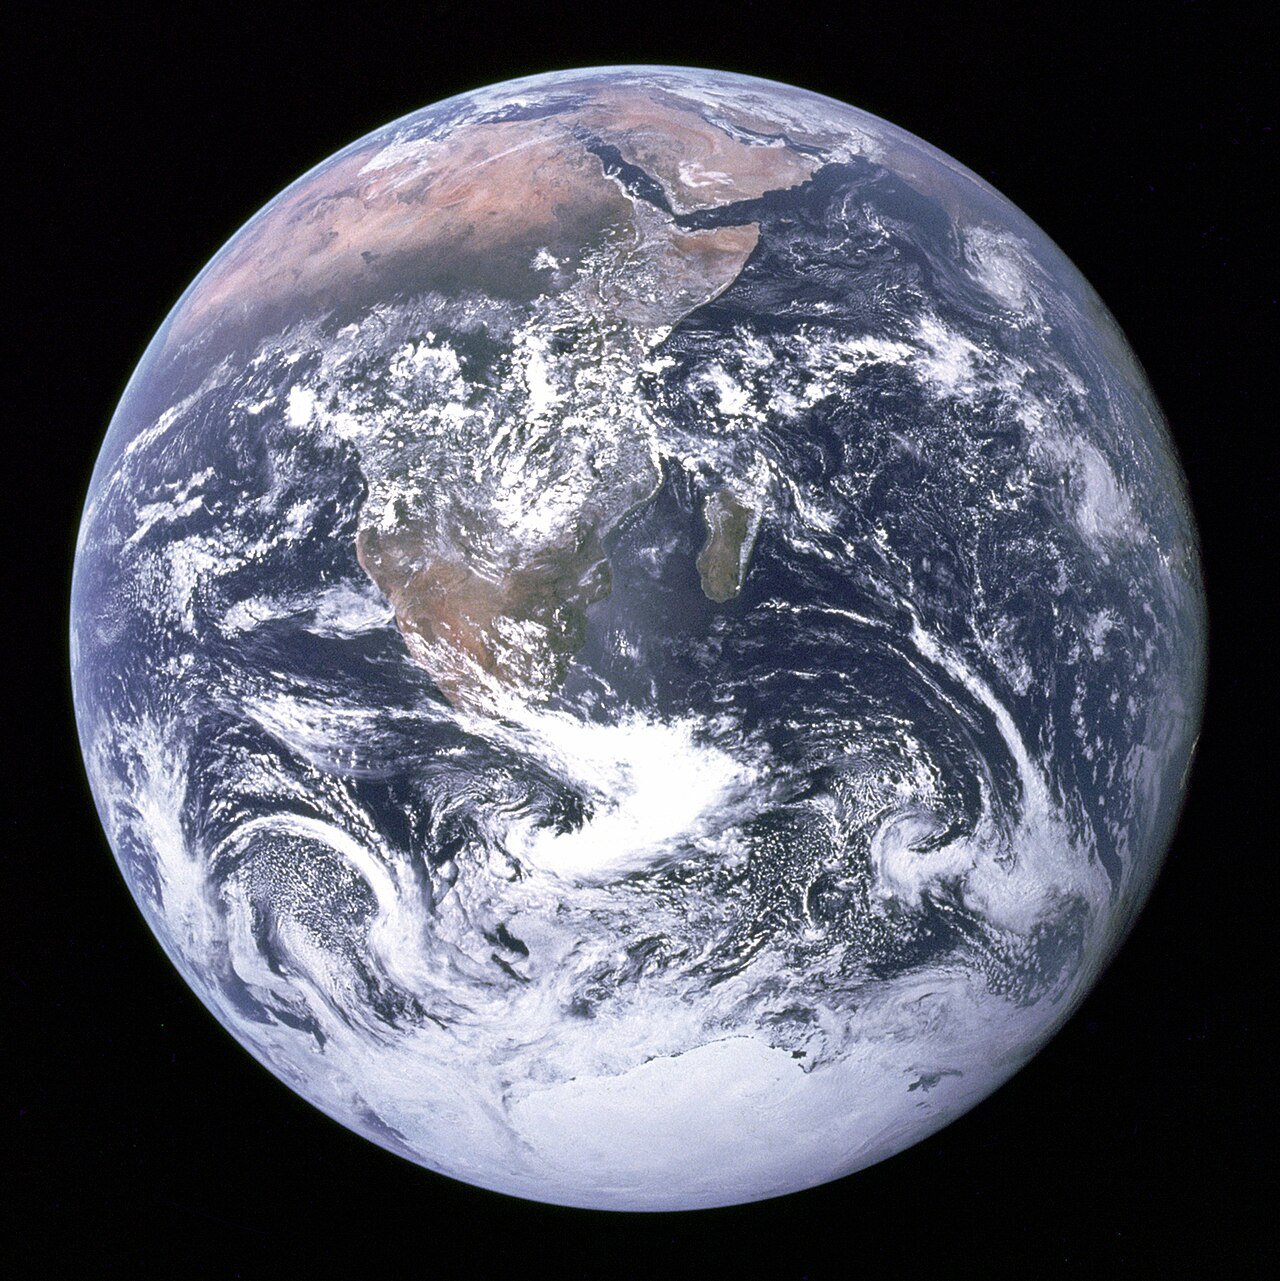
\includegraphics[width=0.5\linewidth]{images/book1/g2-nasa-blue-marble.jpg}

{\small Bumi yang difoto oleh awak Apollo~17, 7~Desember 1972. Kita melihat
Afrika, Jazirah Arab di bagian atas, dan es Antarktika di bagian bawah.
Foto: NASA (domain publik).}
\end{omfigure}

\begin{recall}
Air bisa berwujud padat (es), cair, atau gas yang tidak dapat kita lihat
(uap air). Air cair yang dibiarkan di bawah sinar matahari perlahan-lahan
berubah menjadi uap: air itu menguap. Ketika uapnya mendingin, uap itu
berubah kembali menjadi tetes-tetes yang sangat kecil: uap itu mengembun.
Kamu sudah mengenal perubahan-perubahan ini di buku fisika. Dalam \omterm{def:g1:landscapes-around-us:landscape}{bentang
alam}, air mengalir di \omterm{def:g1:landscapes-around-us:water}{sungai} dan menggenang di \omterm{def:g1:landscapes-around-us:water}{danau}
(\cref{ch:g1:landscapes-around-us}).
\end{recall}

\section{Planet biru}

Sebagian besar Bumi ditutupi air. Bayangkan seluruh permukaan Bumi dipotong
menjadi 100 persegi yang sama besar. Jika kita mewarnai biru setiap persegi
yang ditutupi \omterm{def:g2:water-on-earth:ocean}{laut}, kita mewarnai 71 persegi. Hanya 29 persegi yang berupa
daratan.

\begin{omfigure}
\begin{tikzpicture}
  \begin{axis}[hide axis, width=7.2cm, height=7.2cm, xmin=-0.5, xmax=9.5,
      ymin=-0.5, ymax=9.5, axis equal image, scale only axis,
      clip=false]
    \addplot[scatter, only marks, mark=square*, mark size=9.2pt,
      scatter/classes={0={fill=green!45!omLithAlluv, draw=black!40},
                       1={fill=omSea!80!blue, draw=black!40}},
      point meta=explicit symbolic]
      table[x=col, y=row, meta=blue] {figdata/out/grade-2-ocean_fraction-grid.dat};
  \end{axis}
\end{tikzpicture}

{\small Jika permukaan Bumi dipotong menjadi 100 persegi yang sama besar, 71
di antaranya akan berupa \omterm{def:g2:water-on-earth:ocean}{laut} (biru) dan 29 berupa daratan (hijau). Dihitung
dari peta relief seluruh Bumi (NOAA ETOPO1).}
\label{fig:g2:water-on-earth:grid}
\end{omfigure}
% ledger: data:etopo1, wss:ocean-cover (71 % computed in figdata/grade-2/ocean_fraction.py)

Hamparan \omterm{def:g2:water-on-earth:salt-fresh}{air asin} yang luas, yang menutupi sebagian besar Bumi, mempunyai nama.

\begin{definition}[Samudra dan laut]\label{def:g2:water-on-earth:ocean}
Yang disebut \emph{samudra}\index{samudra} adalah salah satu hamparan \omterm{def:g2:water-on-earth:salt-fresh}{air
asin} yang sangat luas, yang menutupi sebagian besar Bumi dan terletak di
antara benua-benua. Yang disebut \emph{laut}\index{laut} adalah hamparan \omterm{def:g2:water-on-earth:salt-fresh}{air
asin} yang lebih kecil, biasanya di tepi samudra dan sebagian dikelilingi
daratan.
\end{definition}

Semua \omterm{def:g2:water-on-earth:ocean}{samudra} saling bersambung: sebuah kapal bisa berlayar dari \omterm{def:g2:water-on-earth:ocean}{samudra}
mana pun ke \omterm{def:g2:water-on-earth:ocean}{samudra} lainnya tanpa melintasi daratan. Nama-nama \omterm{def:g2:water-on-earth:ocean}{samudra}, dan
letaknya pada bola dunia, ada di \cref{ch:g3:continents-and-oceans}.

\begin{omfigure}
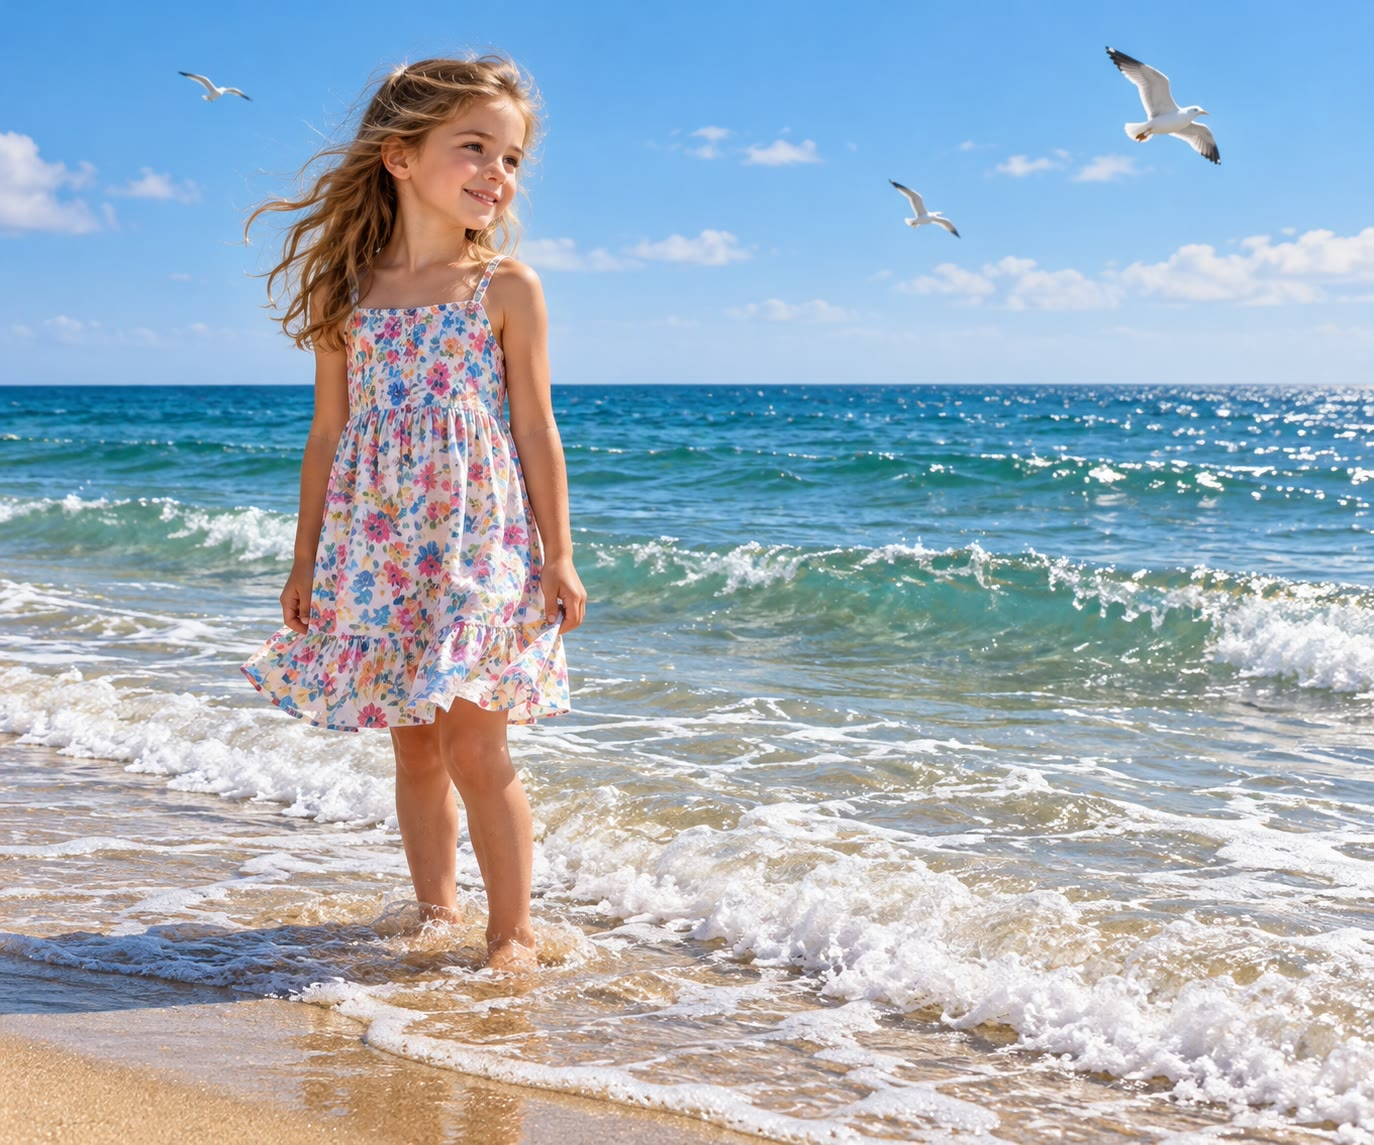
\includegraphics[width=0.62\linewidth]{images/book1/ai/g2-beach-sea.jpg}

{\small Di tepi \omterm{def:g2:water-on-earth:ocean}{laut}. Airnya terus membentang, jauh melampaui batas
pandangan mata.}
\end{omfigure}

\section{Air asin dan air tawar}

Kalau kamu pernah tertelan seteguk air \omterm{def:g2:water-on-earth:ocean}{laut} saat berenang, kamu tahu: air
\omterm{def:g2:water-on-earth:ocean}{laut} terasa sangat asin. Air \omterm{def:g1:landscapes-around-us:water}{sungai} dan \omterm{def:g1:landscapes-around-us:water}{danau} tidak.

\begin{definition}[Air asin dan air tawar]\label{def:g2:water-on-earth:salt-fresh}
Yang disebut \emph{air asin}\index{air asin} adalah air yang di dalamnya
terlarut banyak garam: itulah air \omterm{def:g2:water-on-earth:ocean}{samudra} dan \omterm{def:g2:water-on-earth:ocean}{laut}. Yang disebut
\emph{air tawar}\index{air tawar} adalah air yang garamnya sangat sedikit:
itulah air hujan, air kebanyakan \omterm{def:g1:landscapes-around-us:water}{sungai} dan \omterm{def:g1:landscapes-around-us:water}{danau}, air dari es dan salju,
dan air dari mata air.
\end{definition}

\begin{example}[Seberapa asin laut itu?]\label{ex:g2:water-on-earth:salty}
% ledger: nos:salinity
Dalam sebuah botol berisi satu kilogram air \omterm{def:g2:water-on-earth:ocean}{laut} --- kira-kira satu liter
--- terdapat sekitar 35 gram garam. Jika kita membiarkan semua airnya
menguap, garamnya tertinggal sebagai kristal putih di dasar botol. Begitulah
garam \omterm{def:g2:water-on-earth:ocean}{laut} dibuat di tambak garam di tepi \omterm{def:g2:water-on-earth:ocean}{laut}, tempat sinar matahari dan
angin perlahan-lahan mengeringkan kolam-kolam dangkal berisi air \omterm{def:g2:water-on-earth:ocean}{laut}.
\end{example}

\begin{omfigure}
\begin{minipage}[b]{0.49\linewidth}\centering
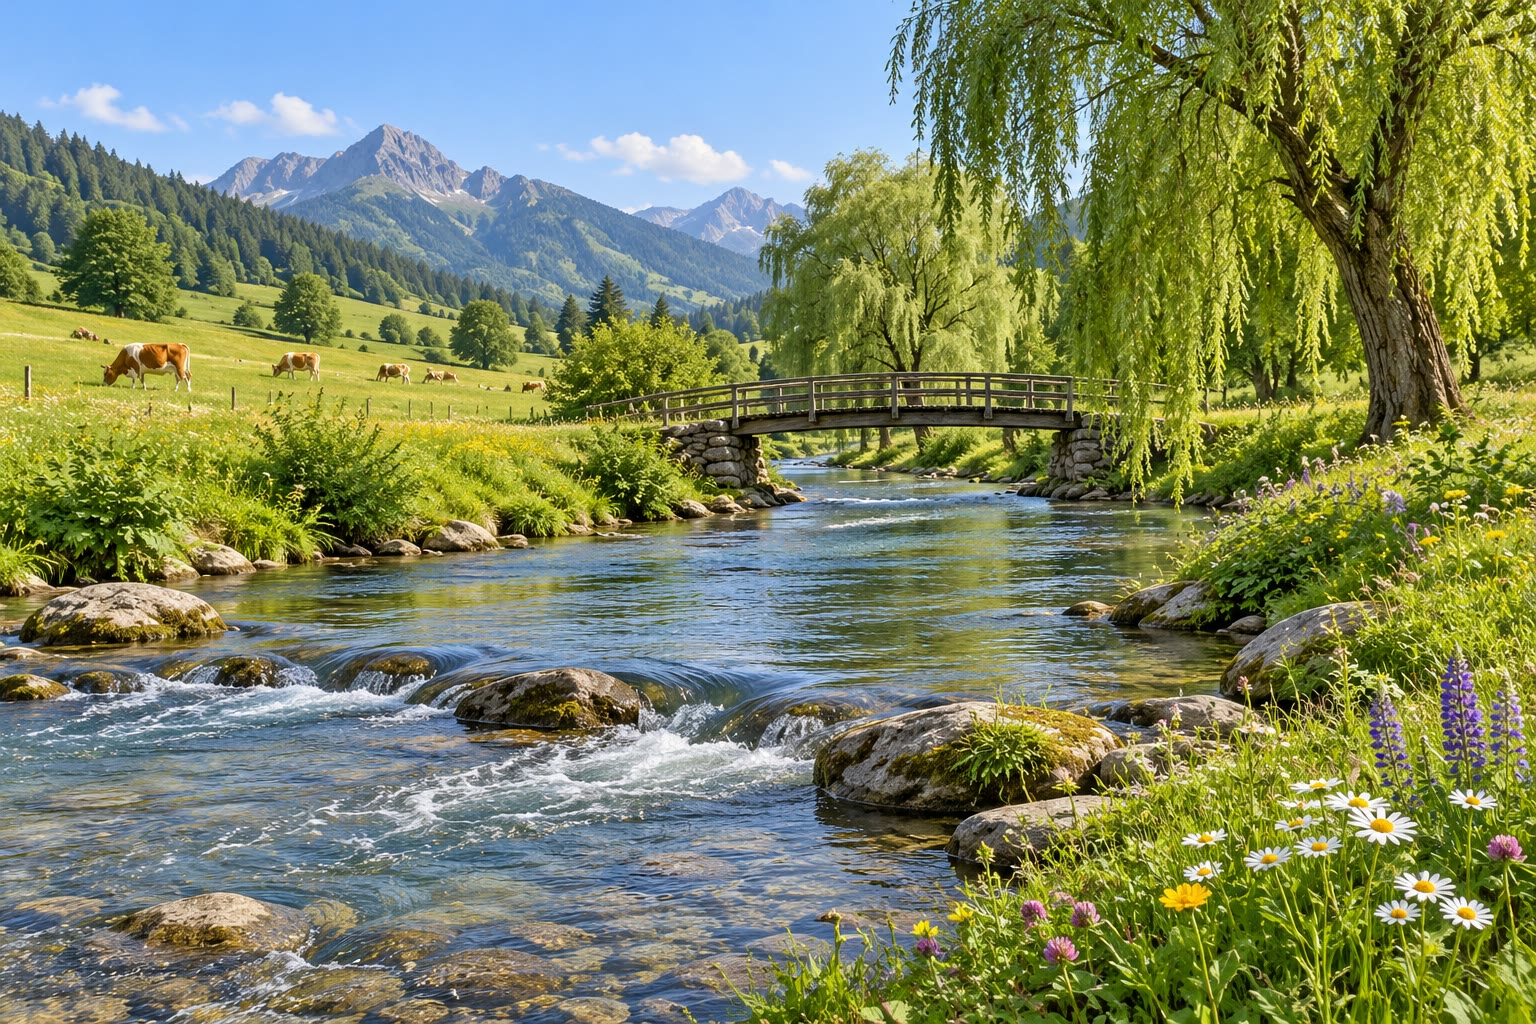
\includegraphics[width=\linewidth]{images/book1/ai/g2-river-meadow.jpg}

{\small \omterm{def:g2:water-on-earth:salt-fresh}{Air tawar}: sebuah \omterm{def:g1:landscapes-around-us:water}{sungai}.}
\end{minipage}\hfill
\begin{minipage}[b]{0.49\linewidth}\centering
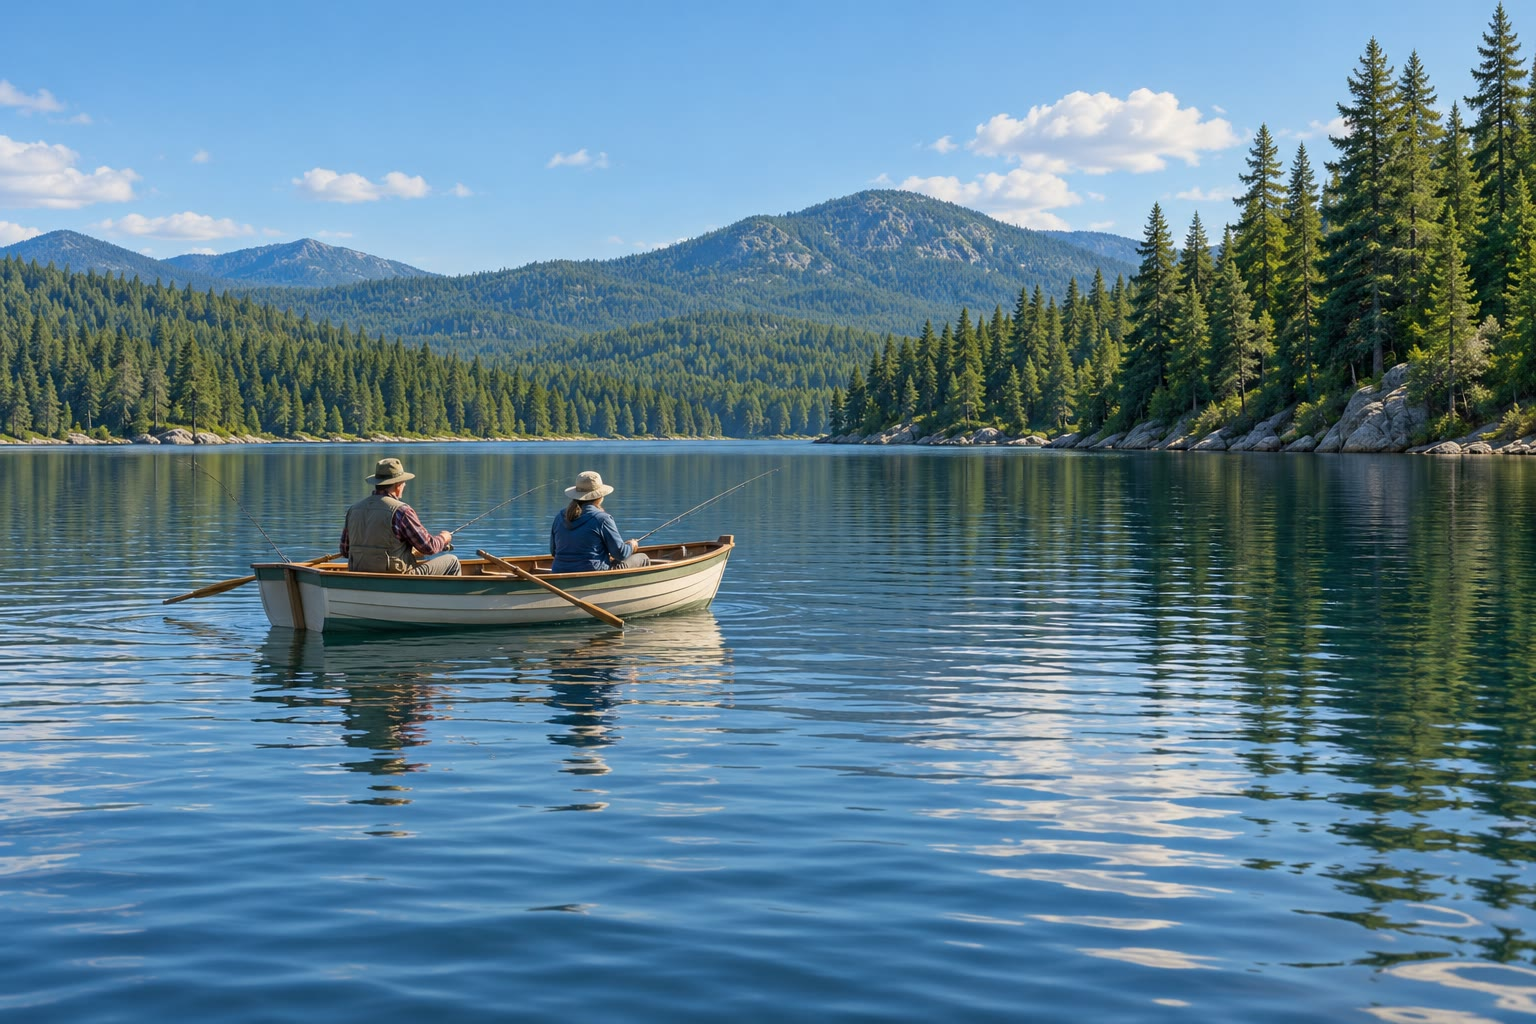
\includegraphics[width=\linewidth]{images/book1/ai/g2-lake-boat.jpg}

{\small \omterm{def:g2:water-on-earth:salt-fresh}{Air tawar}: sebuah \omterm{def:g1:landscapes-around-us:water}{danau}.}
\end{minipage}
\end{omfigure}

\begin{remark}[Kita tidak bisa minum air laut]\label{rem:g2:water-on-earth:drink}
Manusia dan hewan darat tidak bisa minum air \omterm{def:g2:water-on-earth:ocean}{laut}: garamnya terlalu banyak,
dan meminumnya membuat tubuh kehilangan air, bukan mendapat air. Para
pelaut yang berada jauh di tengah \omterm{def:g2:water-on-earth:ocean}{laut}, dikelilingi air, sejak dulu harus
membawa \omterm{def:g2:water-on-earth:salt-fresh}{air tawar} mereka sendiri.
\end{remark}

\section{Di mana semua air itu?}

\omterm{def:g2:water-on-earth:salt-fresh}{Air tawar} tidak hanya ada di \omterm{def:g1:landscapes-around-us:water}{sungai} dan \omterm{def:g1:landscapes-around-us:water}{danau}. Banyak di antaranya membeku:
di dalam es putih yang luas di Antarktika dan Greenland, dan di \omterm{def:g1:landscapes-around-us:landform}{gunung-gunung}
yang tinggi. Banyak pula yang tersembunyi di bawah kaki kita, di dalam tanah,
tempat air itu mengisi celah-celah kecil di antara butir pasir dan
retakan-retakan di batuan.

\begin{omfigure}
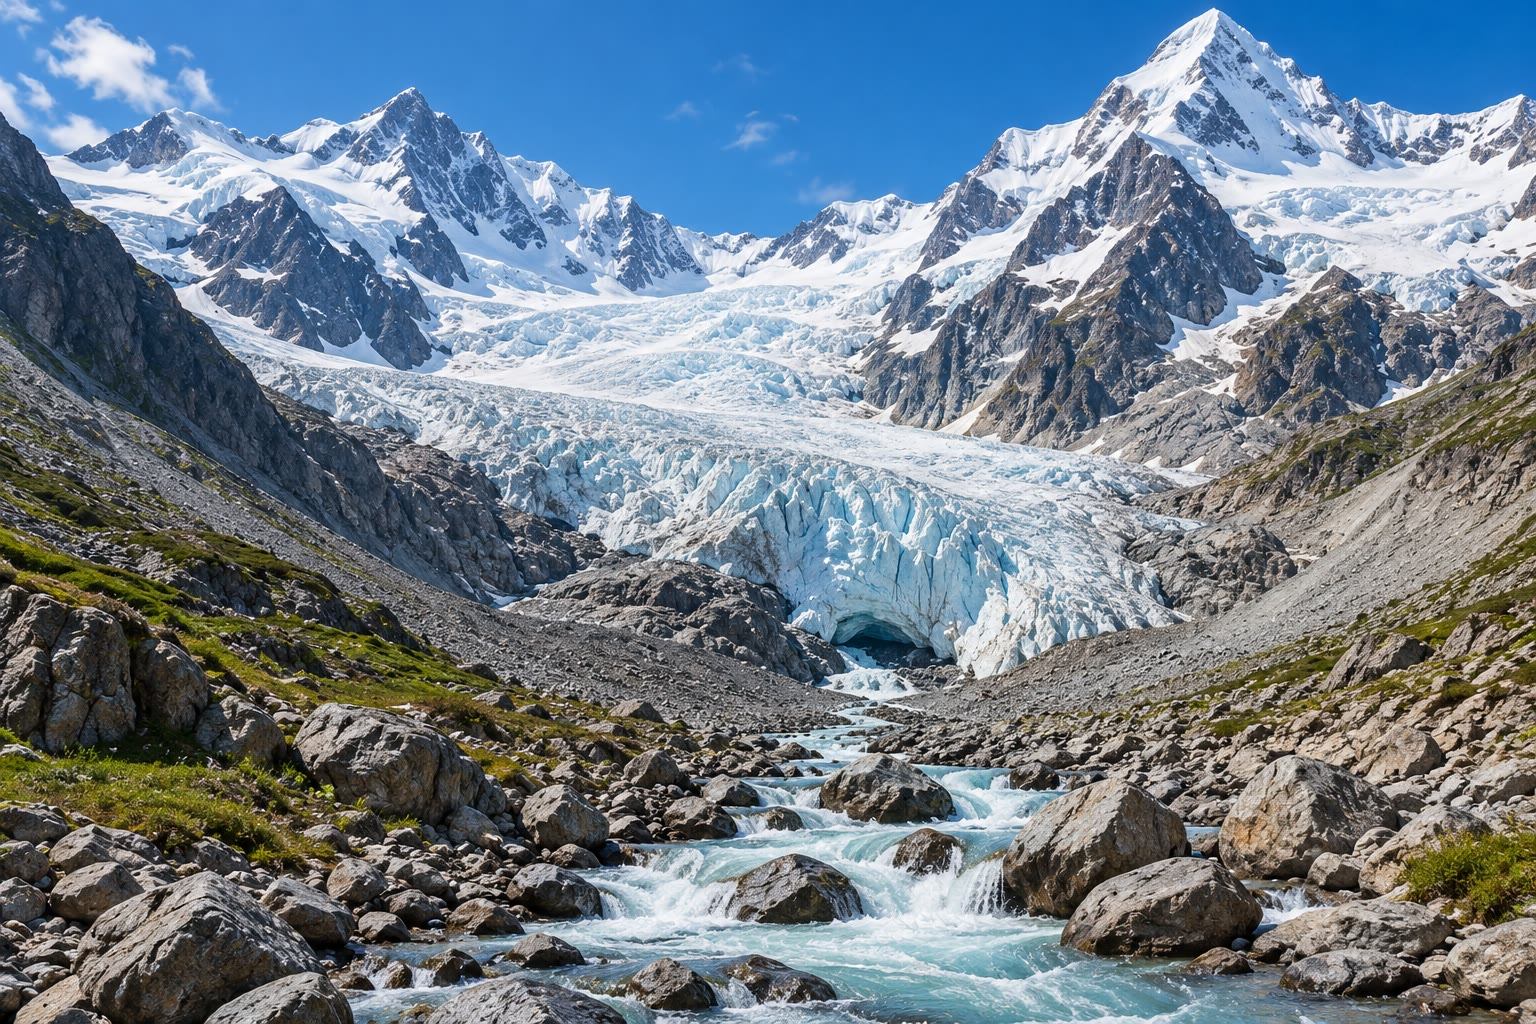
\includegraphics[width=0.62\linewidth]{images/book1/ai/g2-snowy-mountains.jpg}

{\small \omterm{def:g1:landscapes-around-us:landform}{Gunung-gunung} yang tinggi menyimpan \omterm{def:g2:water-on-earth:salt-fresh}{air tawar} sebagai salju dan es
sepanjang tahun. Pada musim panas sebagian mencair dan mengisi \omterm{def:g1:landscapes-around-us:water}{sungai-sungai}
kecil.}
\end{omfigure}

Bayangkan kita bisa menuangkan semua air di Bumi ke dalam 100 ember yang
sama besar. Berapa ember yang akan diisi oleh setiap jenis air?

\begin{omfigure}
\begin{tikzpicture}
  \begin{axis}[hide axis, width=7.2cm, height=7.2cm, xmin=-0.5, xmax=9.5,
      ymin=-0.5, ymax=9.5, axis equal image, scale only axis, clip=false]
    \addplot[scatter, only marks, mark=*, mark size=8pt,
      scatter/classes={0={fill=omSea!80!blue, draw=black!40},
                       1={fill=white, draw=black!60},
                       2={fill=brown!55, draw=black!40}},
      point meta=explicit symbolic]
      table[x=col, y=row, meta=kind] {figdata/out/grade-2-water_shares.dat};
  \end{axis}
  \begin{scope}[shift={(7.9,5.6)}, font=\small]
    \fill[omSea!80!blue, draw=black!40] (0,0) circle (0.2);
    \node[anchor=west] at (0.35,0) {air asin samudra: 96 ember};
    \fill[white, draw=black!60] (0,-0.7) circle (0.2);
    \node[anchor=west] at (0.35,-0.7) {es dan salju: 2 ember};
    \fill[brown!55, draw=black!40] (0,-1.4) circle (0.2);
    \node[anchor=west] at (0.35,-1.4) {air di bawah tanah: 2 ember};
  \end{scope}
\end{tikzpicture}

{\small Semua air di Bumi dalam 100 ember. \omterm{def:g1:landscapes-around-us:water}{Sungai}, \omterm{def:g1:landscapes-around-us:water}{danau}, awan, dan air di
dalam semua makhluk hidup jika digabungkan tidak akan mengisi satu ember
pun. Angka dari U.S. Geological Survey.}
\label{fig:g2:water-on-earth:buckets}
\end{omfigure}
% ledger: wss:water-shares (rounded to 100 buckets in figdata/grade-2/water_shares.py)

\begin{proposition}[Sebagian besar air di Bumi asin]\label{prop:g2:water-on-earth:most-salty}
% ledger: wss:water-shares
Dari 100 ember berisi semua air di Bumi, 96 adalah \omterm{def:g2:water-on-earth:salt-fresh}{air asin} \omterm{def:g2:water-on-earth:ocean}{samudra}. \omterm{def:g2:water-on-earth:salt-fresh}{Air
tawar} yang kita minum hanyalah bagian yang sangat kecil dari seluruh air:
sebagian besar \omterm{def:g2:water-on-earth:salt-fresh}{air tawar} membeku di dalam es, atau tersembunyi di bawah
tanah.
\end{proposition}

\section{Ke mana perginya air hujan?}

Ketika hujan turun, airnya tidak tetap di tempat jatuhnya. Perhatikanlah
halaman sekolah setelah hujan: sebagian air mengalir di atas tanah ke
selokan, sebagian meresap ke dalam tanah di petak-petak bunga, dan
genangan-genangan perlahan-lahan menghilang ketika matahari muncul kembali.

\begin{omfigure}
\begin{tikzpicture}[x=1cm, y=1cm, font=\small]
  % sky, sea, land
  \fill[ocBlue!6] (0,0) rectangle (12,5.6);
  \fill[omSea] (8.6,0) rectangle (12,0.9);
  \fill[green!30!omLithAlluv] (0,0) -- (0,2.4) .. controls (2,2.6) and (3,2.0) .. (4.5,1.6)
     .. controls (6,1.2) and (7.5,1.0) .. (8.6,0.9) -- (8.6,0) -- cycle;
  % ground below the surface
  \fill[brown!25] (0,0) rectangle (8.6,0.6);
  % river
  \draw[omSea!70!blue, line width=2.4pt] (1.6,2.45) .. controls (3.5,2.0) and (6,1.15) .. (8.6,0.95);
  % cloud and rain
  \pic at (2.2,4.0) {puffycloud};
  \foreach \x in {1.4,1.8,2.2,2.6,3.0}
    \draw[omWxRain, line width=0.8pt] (\x,3.7) -- (\x-0.15,3.1);
  \pic at (9.6,4.3) {puffycloud};
  % arrows
  \draw[omWxRain, line width=1.1pt, -{Stealth[length=2.5mm]}] (3.3,2.15) -- (3.3,0.6);
  \node[anchor=west, align=left, font=\scriptsize] at (3.4,1.0) {sebagian meresap\\ke dalam tanah};
  \draw[omWxRain, line width=1.1pt, -{Stealth[length=2.5mm]}] (5.4,1.55) -- (7.6,1.15);
  \node[align=center, font=\scriptsize] at (6.2,2.05) {sebagian mengalir ke sungai,\\dan sungai mengalir ke laut};
  \draw[black!50, line width=1.1pt, densely dashed, -{Stealth[length=2.5mm]}] (10.2,1.1) .. controls (10.4,2.4) and (10.1,3.2) .. (9.8,3.85);
  \node[align=left, anchor=west, font=\scriptsize] at (10.45,2.4) {air\\menguap};
  \draw[black!50, line width=1.1pt, densely dashed, -{Stealth[length=2.5mm]}] (8.45,4.35) -- (3.6,4.3);
  \node[font=\scriptsize, above] at (6.0,4.35) {angin membawa awan-awan};
  \node[font=\scriptsize] at (10.4,0.45) {laut};
  \node[font=\scriptsize, anchor=west] at (0.2,3.25) {hujan};
\end{tikzpicture}

{\small Ke mana air hujan pergi. Air yang naik dari \omterm{def:g2:water-on-earth:ocean}{laut} dan dari daratan
sebagai uap membentuk awan-awan baru, dan awan-awan itu membawa hujan baru.}
\label{fig:g2:water-on-earth:rain}
\end{omfigure}

\begin{method}[Mengikuti setetes air hujan]\label{met:g2:water-on-earth:drop}
Untuk mengikuti setetes air hujan, ajukan tiga pertanyaan secara berurutan:
\begin{enumerate}
  \item Di mana tetes itu jatuh: di \omterm{def:g2:water-on-earth:ocean}{laut}, di atap, di tanah, di \omterm{def:g1:landscapes-around-us:landform}{gunung}?
  \item Apakah tetes itu meresap ke dalam tanah, mengalir di atas
        permukaan, atau membeku menjadi es?
  \item Ke mana tetes itu pergi sesudahnya: ke \omterm{def:g1:landscapes-around-us:water}{sungai}, ke \omterm{def:g1:landscapes-around-us:water}{danau}, ke \omterm{def:g2:water-on-earth:ocean}{laut},
        ke dalam tanah, atau kembali ke udara?
\end{enumerate}
Pada akhirnya, setiap tetes kembali ke \omterm{def:g2:water-on-earth:ocean}{laut} atau ke udara, dan perjalanannya
dimulai lagi.
\end{method}

\begin{example}[Setetes air di gunung]\label{ex:g2:water-on-earth:mountain}
Setetes air hujan jatuh sebagai salju di sebuah \omterm{def:g1:landscapes-around-us:landform}{gunung} yang tinggi pada
musim dingin. Tetes itu tinggal di sana, membeku, sampai hari-hari hangat
di musim panas. Lalu tetes itu mencair, mengalir turun ke \omterm{def:g1:landscapes-around-us:water}{sungai} kecil di
pegunungan, bergabung dengan sebuah \omterm{def:g1:landscapes-around-us:water}{sungai}, dan \omterm{def:g1:landscapes-around-us:water}{sungai} itu membawanya ke
\omterm{def:g2:water-on-earth:ocean}{laut}. Pada suatu hari yang cerah, tetes itu menguap dari \omterm{def:g2:water-on-earth:ocean}{laut} dan naik ke
udara, tempat ia menjadi bagian dari awan yang baru.
\end{example}

\section{Latihan}

\begin{exercise}[$\star$]\label{exo:g2:water-on-earth:1}
\omterm{def:g2:water-on-earth:salt-fresh}{Air asin} atau \omterm{def:g2:water-on-earth:salt-fresh}{air tawar}? \omterm{def:g2:water-on-earth:ocean}{Laut}; \omterm{def:g1:landscapes-around-us:water}{sungai}; hujan; \omterm{def:g1:landscapes-around-us:water}{danau} di pegunungan;
\omterm{def:g2:water-on-earth:ocean}{samudra}; es di \omterm{def:g1:landscapes-around-us:landform}{gunung}.
\end{exercise}

\begin{exercise}[$\star$]\label{exo:g2:water-on-earth:2}
Mengapa Bumi kita sebut ``planet biru''?
\end{exercise}

\begin{exercise}[$\star$]\label{exo:g2:water-on-earth:3}
Pada kisi 100 persegi, 71 persegi berwarna biru. Berapa persegi yang berupa
daratan?
\end{exercise}

\begin{exercise}[$\star$]\label{exo:g2:water-on-earth:4}
Mana yang lebih besar, \omterm{def:g2:water-on-earth:ocean}{samudra} atau \omterm{def:g2:water-on-earth:ocean}{laut}?
\end{exercise}

\begin{exercise}[$\star$]\label{exo:g2:water-on-earth:5}
Dapatkah seorang pelaut di tengah \omterm{def:g2:water-on-earth:ocean}{samudra} meminum air di sekeliling
kapalnya? Mengapa?
\end{exercise}

\begin{exercise}[$\star$]\label{exo:g2:water-on-earth:6}
Sebutkan tiga tempat \omterm{def:g2:water-on-earth:salt-fresh}{air tawar} dapat ditemukan.
\end{exercise}

\begin{exercise}[$\star\star$]\label{exo:g2:water-on-earth:7}
Pada gambar 100 ember, berapa ember yang berisi \omterm{def:g2:water-on-earth:salt-fresh}{air asin}? Berapa ember
yang berisi \omterm{def:g2:water-on-earth:salt-fresh}{air tawar} (es dan air di bawah tanah digabungkan)?
\end{exercise}

\begin{exercise}[$\star\star$]\label{exo:g2:water-on-earth:8}
Urutkan dari yang menyimpan air paling banyak sampai yang paling sedikit:
\omterm{def:g1:landscapes-around-us:water}{sungai-sungai}; \omterm{def:g2:water-on-earth:ocean}{samudra-samudra}; es dan salju.
\end{exercise}

\begin{exercise}[$\star\star$]\label{exo:g2:water-on-earth:9}
Hujan turun di sebuah ladang. Sebutkan dua hal yang bisa terjadi pada airnya.
\end{exercise}

\begin{exercise}[$\star\star$]\label{exo:g2:water-on-earth:10}
Sebuah panci berisi air \omterm{def:g2:water-on-earth:ocean}{laut} dibiarkan di bawah sinar matahari selama
berhari-hari, sampai airnya habis. Apa yang tertinggal di dasar panci? Ke
mana perginya air itu?
\end{exercise}

\begin{exercise}[$\star\star$]\label{exo:g2:water-on-earth:11}
Ceritakan perjalanan setetes air hujan yang jatuh di atap sekolah, sampai
tetes itu kembali berada di dalam awan.
\end{exercise}
